\subsection{Class Diagram}

The following is the class diagram of the project, divided in the main five parts.

\subsubsection{Resources}

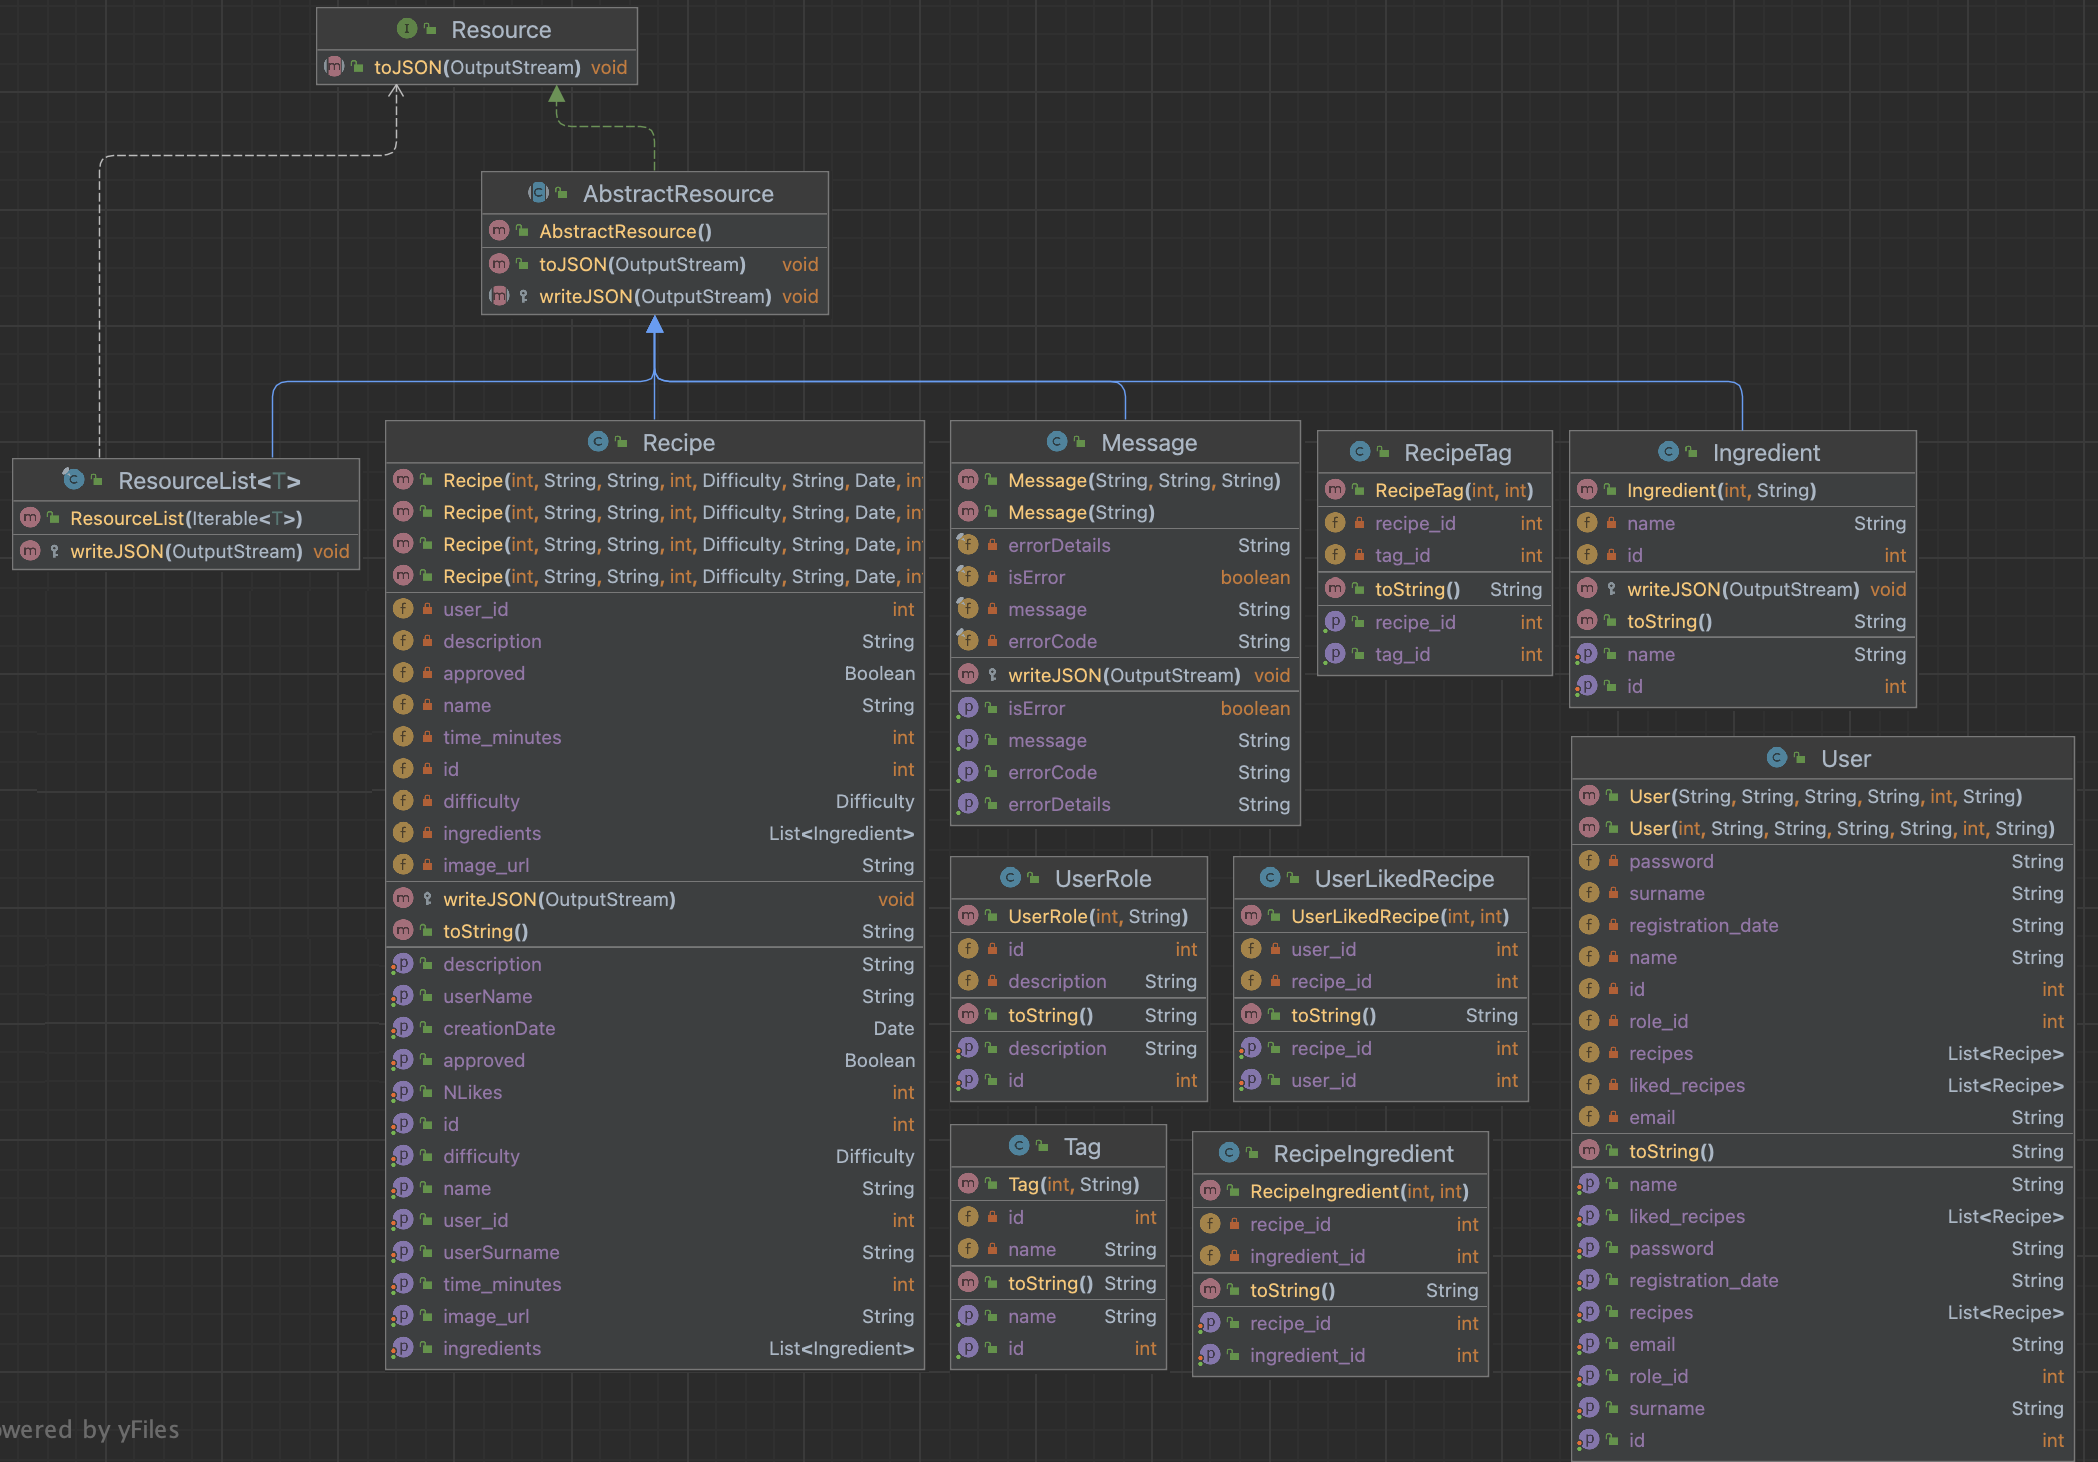
\includegraphics[width=\textwidth]{images/resources.png}

These are the classes that represent the objects mapped from/to the database tables, also the relation tables. For example, the class "Recipe" reflects the "Recipe" table, having the same fields plus methods. They all are subclasses of the class "Resource", that implements the definition of the "toJSON" method.

\subsubsection{DAOs}

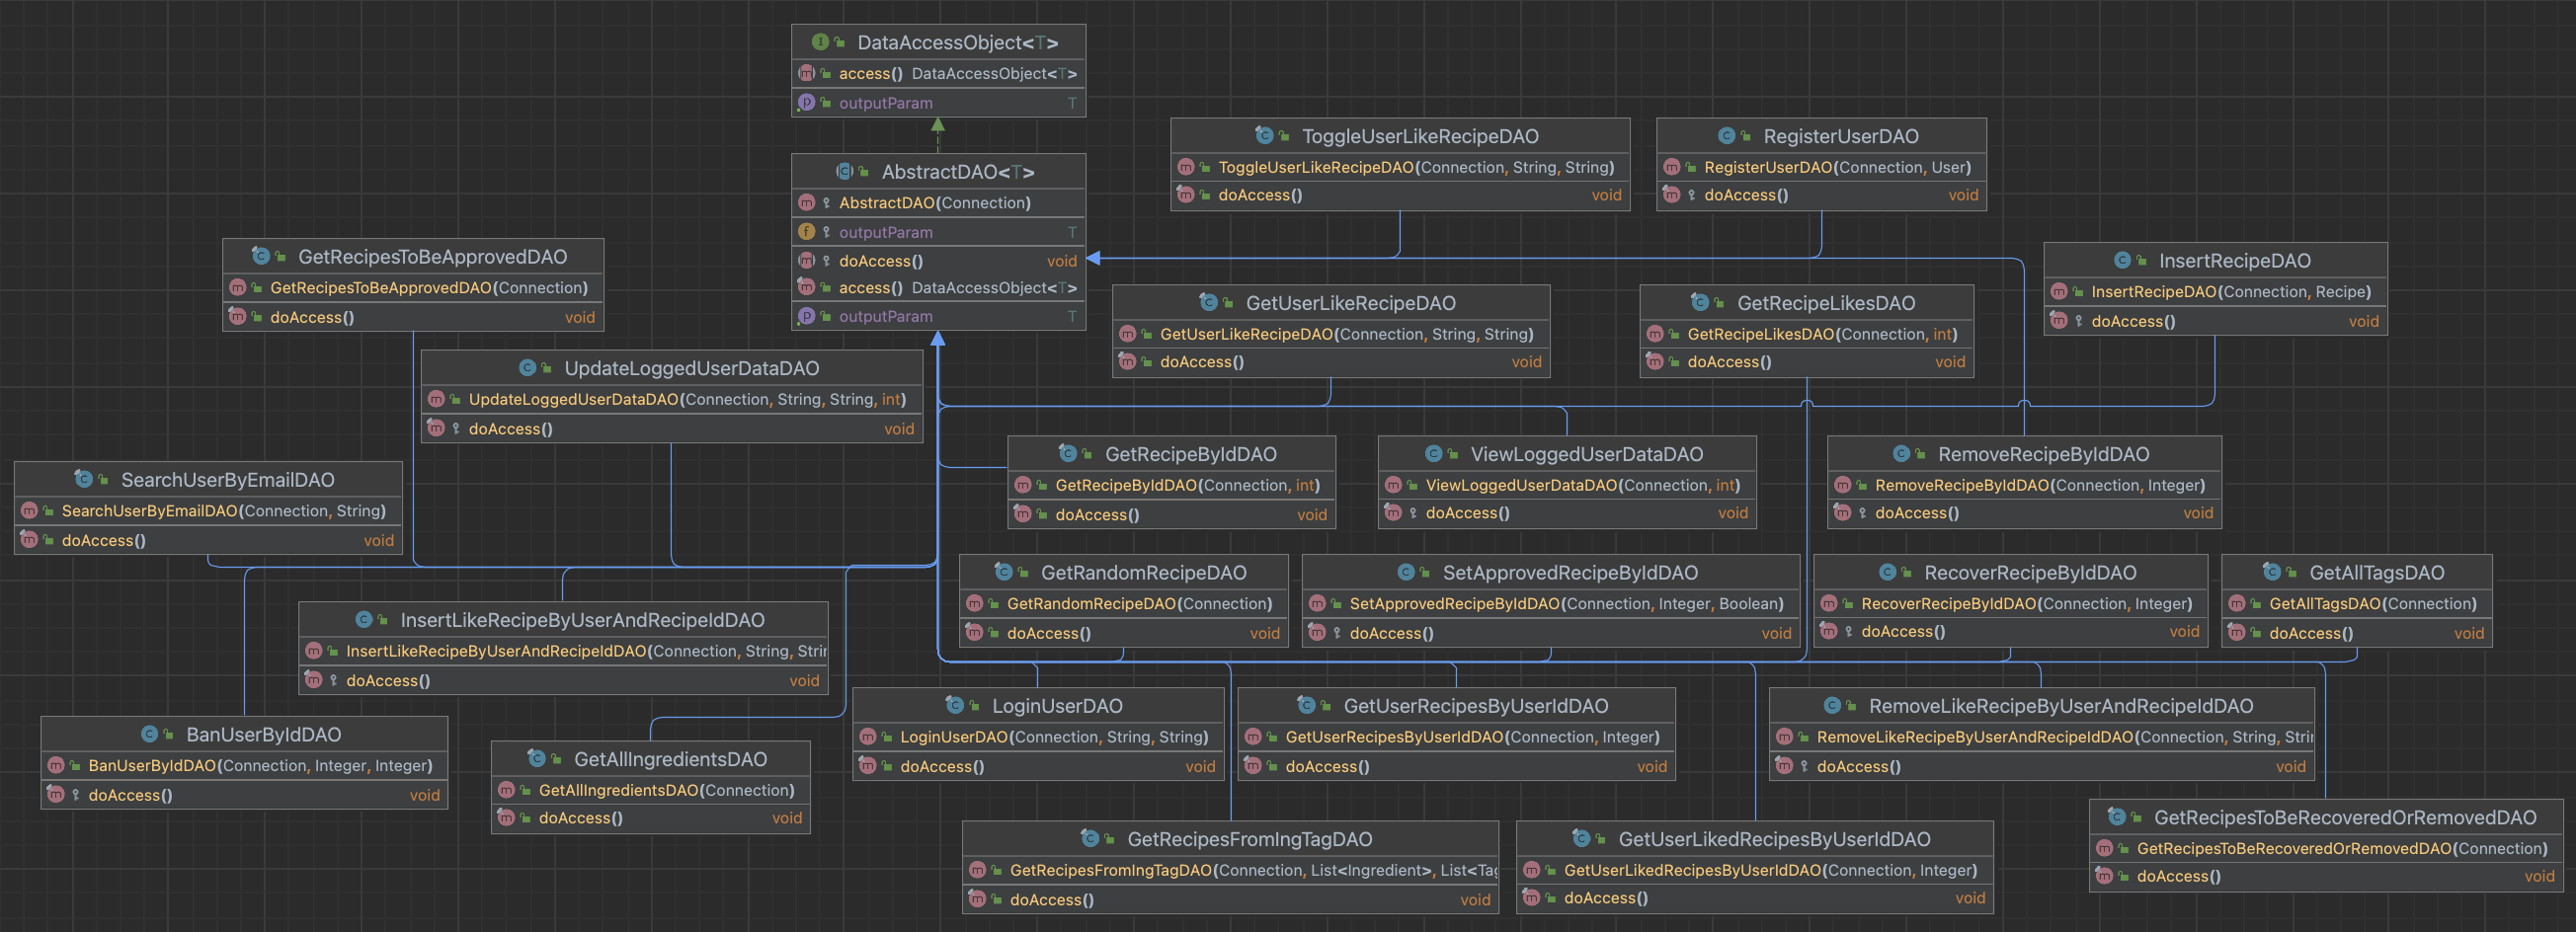
\includegraphics[width=\textwidth]{images/dao.png}

The DAOs are the classes used to access the database and perform an atomic action. For example the action of creating a recipe is done in the "InsertRecipeDAO", that takes an input a "Recipe" and a "Connection" and saves it on the database. Necessary checks for errors are of course done. All DAOs are subclasses of "AbstractDAO", which defines the "doAccess" method, that handles the access to the database with a "Connection" and the subsequent closure.

\subsubsection{Servlets}

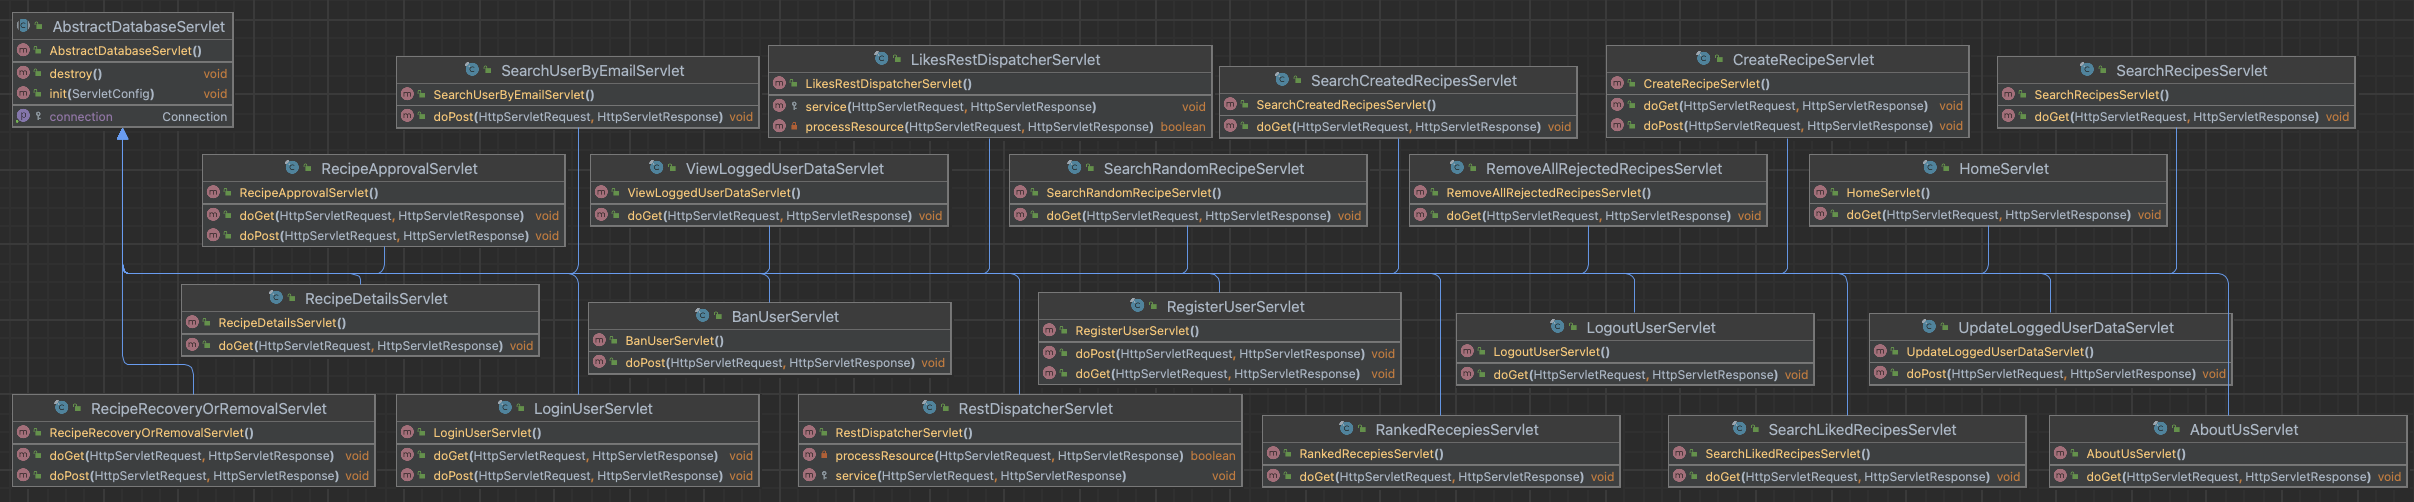
\includegraphics[width=\textwidth]{images/servlets.png}
Servlets are used the intermediary between the client and the server by handling HTTP requests and generating appropriate HTTP responses. Each servlet corresponds to a particular URL pattern (all configured in "WEB.xml" file) and performs specific tasks based on the request parameters, also handling POST requests in the "doPost" method and the GET ones i the "doGet" method. For instance, the "SearchRandomRecipeServlet" manages requests of type GET with the appropriate URL and redirects the user to the page of a random recipe.






\subsubsection{REST}

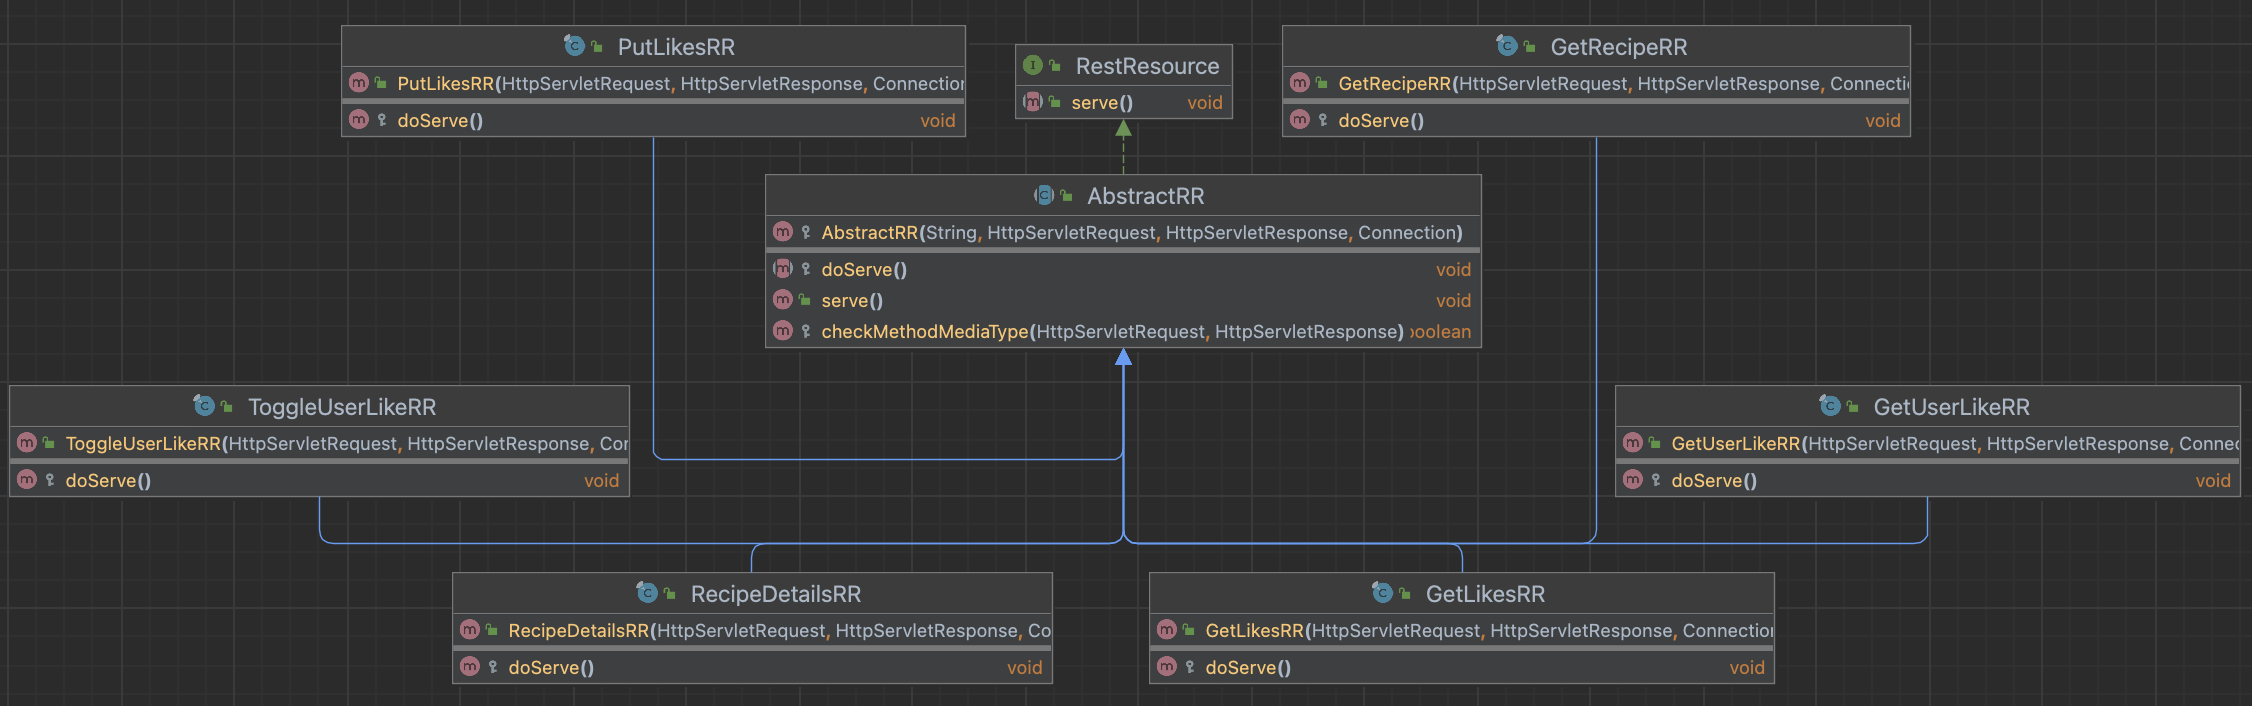
\includegraphics[width=\textwidth]{images/rest.png}
The classes used to manage the REST APIs, discussed later.



\subsubsection{Other}

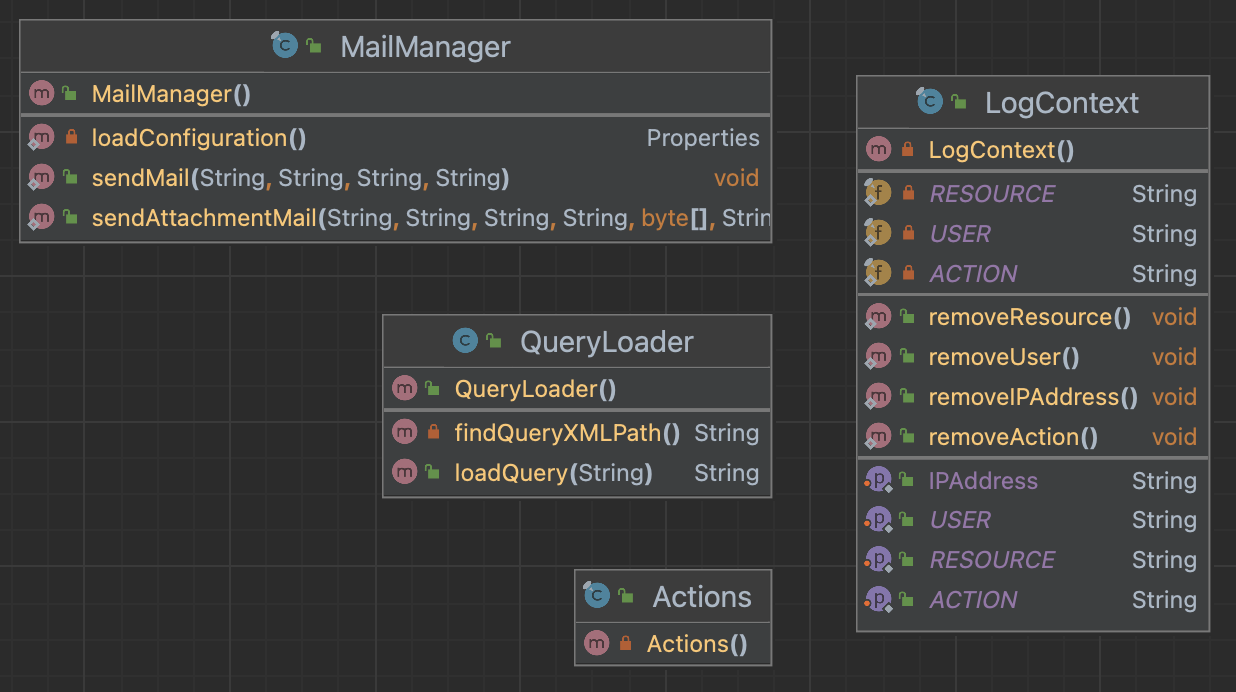
\includegraphics[width=\textwidth]{images/other.png}
These are other tools/utils that have been used in the project.
\begin{itemize}
    \item LogContext: used to store some user information when the user is trying to do a specific action, to be later logged into the web app logs. For example when a user logs in, we log the ip address, the time and other information of the user.
    \item Actions: class that defines a series of actions (strings) that are used in "LogContext" to explicitly log what action the user is actually doing.
    \item QueryLoader: Queries are stored in an external file. This class serves the DAOs and loads the specific query they need.
    \item MailManager: class that manages the sending of emails to users.

\end{itemize}